\documentclass[french]{report}
\usepackage[T1]{fontenc}
\usepackage[utf8]{inputenc}
\usepackage{lmodern}
\usepackage[a4paper]{geometry}
\usepackage{graphicx}
\usepackage{siunitx}
\usepackage{multirow}
\usepackage{xcolor}
\usepackage{fancyhdr}
\usepackage{mathtools}
\usepackage{amssymb}
\usepackage{pgfplots}
\usepackage{babel}
\usepackage{listings}
\usepackage{hyperref} %doit etre défini en dernier !

%en-tetes
\pagestyle{fancy}
\fancyhead[L]{UO \LaTeX}

\newcommand{\lang}{Java}
\newcommand{\attention}[1]{{\color{red}\textbf{ATTENTION: #1}}}
\newcommand{\baremenote}[3]{Note supérieure ou égale à \num{#1} et strictement inférieure à \num{#2} : #3}
\newcommand{\voirparagraphe}[1]{voir paragraphe~\no~\ref{#1}, page~\pageref{#1}}
\newcommand{\nomfichier}[1]{\texttt{#1}}
\newcommand{\refexemple}[1]{(exemple~\ref{#1} page~\pageref{#1})}
\newcommand{\reffigure}[1]{(figure~\ref{#1} page~\pageref{#1})}
\newtheorem{exemple}{Exemple}[section]
\newtheorem{definition}{Définition}
\newtheorem{remarque}{Remarque}

\DeclareSIUnit{\byte}{B}
\DeclareSIUnit{\bit}{bit}

\sisetup{locale=FR}

\lstset{aboveskip=1ex, frame=single, framesep=2pt, language=Java, basicstyle=\ttfamily, breaklines, keywordstyle=\color{blue}, commentstyle=\color{gray}\itshape, stringstyle=\color{orange}}

\title{UO \LaTeX{} - Programmer en \lang{}}
\author{Thomas BOCQUELET}
\date{
	\today{}
	\begin{center}
		\includegraphics[width=0.3\linewidth]{images/logoulco}
	\end{center}
}

\begin{document}
	\maketitle
	
	\begin{abstract}
		Ce document a été réalisé à partir du cours (datant de 2017) de M\up{r} Grégory \bsc{Bourgin}, enseignant-chercheur et Maître de conférence à l'Université du Littoral Côte d'Opale.
		
		\begin{description}
			\item[Email:] bourguin@lisic.univ-littoral.fr
			\item[Page internet:] \url{http://www-lisic.univ-littoral.fr/spip.php?article50\&membre=10}
		\end{description}
		
	\end{abstract}
	
	\tableofcontents
	\listoffigures
	\listoftables
	
	% chapitres du rapport
	
	\section{Présentation}

	\subsection{Qu'est-ce que le Java ?}
	
		\begin{frame}
			\frametitle{Présentation}
			\framesubtitle{Qu'est-ce que le Java ?}
			\begin{block}{Histoire}
				\begin{itemize}[<+->]
					\item Alan \bsc{Key} conçoit le langage \og SmallTalk\fg{} qui est encore \emph{la} référence dans les langages orientés objets.
					\item Création de nombreuses extensions objet pour le C, C++, Object Pascal, etc.
					\item Au milieu des années 90, Sun publie Java.
				\end{itemize}
			\end{block}
		\end{frame}
	
		\begin{frame}
			\frametitle{Présentation}
			\framesubtitle{Qu'est-ce que le Java ?}
			Le Java est:
			\begin{itemize}[<+->]
				\item un langage orienté objet (POO\footnote{Programmation Orientée Objet})
				\item une architecture\emph{Virtual Machine}
				\item un ensemble d'\emph{API} variées
				\item un ensemble d'outils: le \emph{JDK}\footnote{Java Development Kit}
				\item portable
					\begin{itemize}
						\item \emph{JVM}\footnote{Java Virtual Machine} présente sur systèmes Windows, Mac et Unix
						\item accompagné d'une librairie standard
					\end{itemize}
				\item robuste
					\begin{itemize}
						\item mécanisme d'\emph{exceptions}
					\end{itemize}
			\end{itemize}
		\end{frame}	
	
		\begin{frame}
			\frametitle{Présentation}
			\framesubtitle{Qu'est-ce que le Java ?}
			\begin{alertblock}{Attention !}
				\begin{itemize}
					\item <1-> Le Java n'est pas du JavaScript. Le Java est un langage \og généraliste\fg{}, contrairement au JavaScript qui est orienté sur la programmation Web.
					\item <2-> Le Java n'est pas du C++. Java est un langage \emph{purement} objet et de plus haut niveau.
				\end{itemize}
			\end{alertblock}
		\end{frame}	
	
	\subsection{Les outils}
	
		\begin{frame}
			\frametitle{Présentation}
			\framesubtitle{Les outils}
			Environnements de développement:
			\begin{itemize}
				\item SunJDK
				\item Eclipse
				\item IntelliJ (version \og community\fg{} gratuite, commerciale payante)
				\item NetBeans
			\end{itemize}
			\pause
			\begin{remarque}
				Dans les TPs, nous utiliserons les environnements de développement IntelliJ et Eclipse.
			\end{remarque}
		\end{frame}	
	
		\begin{frame}
			\frametitle{Présentation}
			\framesubtitle{Les outils}
			Liste des outils de Java:
			\begin{description}
				\item[javac:] compilateur de sources Java
				\item[java:] interpréteur de byte code
				\item[appletviewer:] interpréteur d'applet
				\item[javadoc:] générateur de documentation (HTML, MIF)
				\item[javah:] générateur de header pour l'appel de méthodes natives
				\item[javap:] désassembleur de byte code
				\item[jdb:] debugger
				\item[javakey:] générateur de clés pour la signature de code
			\end{description}
		\end{frame}	
	
		\begin{frame}
			\frametitle{Présentation}
			\framesubtitle{Les outils}
			Liste des \emph{API} standards:
			\begin{description}
				\item[java.lang:] types de bases, etc.
				\item[java.util:] HashTable, Vector, Stack, Date...
				\item[java.io:] accès aux entrées/sorties par flux
				\item[java.net:] socket, URL...
				\item[java.sql:] accès homogène aux bases de données
				\item[java.security:] signatures, cryptographie, authentification...
			\end{description}
		\end{frame}	
	
	
	\subsection{Références}
	
		\begin{frame}
			\frametitle{Présentation}
			\framesubtitle{Références}
			Java dispose d'un grand nombre de ressources sur internet.
			
			La version actuelle de Java est la \no 8.
			
			\begin{block}{Documentation officielle}
				\url{https://docs.oracle.com/javase/8/}
			\end{block}
		\end{frame}	

	\chapter{Les éléments du langage}
		\section{Les types primitifs}
		
			\begin{table}[h]
	\centering
	\begin{tabular}{|c|c|c|c|m{5cm}|}
		\hline 
			Type & Taille & Valeur minimale & Valeur maximale & Exemple \\
		\hline
			\lstinline|byte| & \SI{8}{\bit} &\num{-128} & \num{127} & \lstinline|byte b = 64;| \\
		\hline 
			\lstinline|char| & \SI{16}{\bit} & \num{0} &$ 2^{16}-1 $& \lstinline|char c = 'A'; char d = 64;| \\
		\hline 
			\lstinline|short| & \SI{16}{\bit} & $ -2^{15}$ & $ 2^{15}-1 $ &  \lstinline|short s = 65;| \\
		\hline 
			\lstinline|int| & \SI{32}{\bit} & $ -2^{31}$ & $ 2^{31}-1 $ & \lstinline|int i = 1;| \\
		\hline
			\lstinline|long| & \SI{64}{\bit} & $ -2^{63}$ & $ 2^{63}-1 $ & \lstinline|long i = 65L;| \\
		\hline
			\lstinline|float| & \SI{32}{\bit} & $ -2^{-149}$ & $ 2-2^{-23} \times 2^{127} $ & \lstinline|float f = 65f;| \\
		\hline
			\lstinline|double| & \SI{64}{\bit} & $ -2^{-1074}$ & $ 2-2^{-52} \times 2^{1023} $ & \lstinline|double d = 65.55;| \\
		\hline
			\lstinline|boolean| & \SI{1}{\bit} & & & \lstinline|boolean b = true;| \lstinline|boolean c = false;| \\
		\hline
			\lstinline|void| & & & & \\
		\hline
	\end{tabular} 
	\caption{Tableau des types primitifs}
	\label{tableautypesprimitifs}
\end{table}
		
		\section{Les variables}
		
			En \lang, les variables sont typées, et peuvent être déclarées dans n'importe quel bloc du code.
			\begin{exemple}
				On considère le code suivant:
				\lstinputlisting{code/porteevariables.java}
			\end{exemple}
			\textbf{Résultat:} La variable \lstinline|x| sera utilisable dans les blocs 1, 2 et 3.
			La variable \lstinline|y| ne sera utilisable que dans le bloc 2.
			
			Liste des opérateurs d'affectation:
			\begin{itemize}
				\item \lstinline|=|
				\item \lstinline|+=|
				\item \lstinline|-=|
				\item \lstinline|*=|
				\item \lstinline|/=|
				\item \lstinline|%=|
			\end{itemize}
		
		\section{Expressions}
		
			\begin{definition}[Expression ternaire]
				Une \emph{expression ternaire} est une notation \og simplifiée\fg{} d'un test logique.
			\end{definition}
			\begin{exemple}
				Test classique
				\lstinputlisting{code/testClassique.java}
			\end{exemple}
			\begin{exemple}
				Test sous forme d'opérateur ternaire
				\lstinputlisting{code/operateurTernaire.java}
			\end{exemple}
		
			\begin{definition}[Type casting]
				Il est nécessaire de \emph{caster} des affectations lorsque celles-ci ne sont pas implicites, sinon des erreurs de compilation sont détectées.
				\lstinputlisting{code/cast.java}
			\end{definition}
		
		\begin{remarque}
			Levé d'ambiguité entre \lstinline|float| et \lstinline|double|
			\lstinputlisting{code/floatdouble.java}
		\end{remarque}
		
		\section{Les méthodes}
		
			\begin{definition}
				Une \emph{méthode} est une \emph{fonction} appartenant à une \emph{classe}.
			\end{definition}
			Une \emph{méthode} se définit comme suit:
			\lstinputlisting{code/basemethode.java}
			
			\begin{remarque}
				Le type de retour est un type primitif, une classe ou \lstinline|void|.
			\end{remarque}
			\begin{remarque}
				La liste des paramètres peut être vide.
			\end{remarque}
			\begin{remarque}
				Si le type de retour n'est pas un \lstinline|void|, la fonction doit se terminer par un \lstinline|return|.
			\end{remarque}
	
			Passage de paramètres:
				\begin{itemize}
					\item Les paramètres de type simple (\lstinline|int|, \lstinline|float|) sont passés par valeur uniquement
					\item Les paramètres de type \emph{objet} ou tableau sont passés par \emph{référence}
				\end{itemize}
		
		\section{Les structures de contrôle}
		
			\subsection{Si (\lstinline{if})} \label{if}
			
				Le code à l'intérieur d'un \lstinline|if| s'exécute uniquement si la condition est vraie.
				
				\attention{Plusieurs notations sont possibles ! Soyez vigilants au nombre de lignes de code dans votre bloc d'instructions (si votre condition est vraie) pour bien choisir la notation.}
			
				Différentes notations:
				\begin{itemize}
					\item \lstinline|if(condition) {...} else {...}|
					\item \lstinline|if(condition) instruction;|
					\item \lstinline|if(condition) instruction; else instruction;|
					\item \lstinline|if(condition) instruction; else {...}|
					\item \lstinline|if(condition) {...} else instruction;|
				\end{itemize}
			
				\begin{exemple}
					Exemple d'un test simple, avec deux notations différentes:
					\lstinputlisting{code/exempleIF.java}
				\end{exemple}
			
			\subsection{Tant que (\lstinline|while|)}
			
				Le code à l'intérieur d'un \lstinline|while| s'exécute \emph{tant que} la condition est vraie.
			
				\begin{remarque}
					Comme pour le \lstinline|if| (\voirparagraphe{if}), il existe plusieurs notations possibles.
				\end{remarque}
			
				Différentes notations:
				\begin{itemize}
					\item \lstinline|while(condition) {...}|
					\item \lstinline|while(condition) instruction;|
				\end{itemize}
			
				\begin{exemple}
					Exemple d'une boucle qui affiche les chiffres de \num{0} à \num{9}:
					\lstinputlisting{code/exempleWHILEsansDO.java}
				\end{exemple}
			
				\begin{remarque}
					Le \lstinline|while|, tel que définit jusqu'à présent, vérifie la condition avant d'exécuter (au moins une fois) les instructions. Dans certains cas, il pourrait être utile d'exécuter les instructions une première fois, avant de vérifier si la condition est vraie: on utilisera \lstinline|do|.
				\end{remarque}
			
				\begin{exemple}
					Exemple d'une boucle qui affiche également les chiffres de \num{0} à \num{9}:
					\lstinputlisting{code/exempleWHILEavecDO.java}
				\end{exemple}
				
				\textbf{Explication du fonctionnement:}
					\begin{enumerate}
						\item A la 1\iere{} exécution, le code à l'intérieur du bloc \lstinline|do| sera exécuté: \lstinline|i| vaudra donc \num{1}
						\item Puisque la condition du \lstinline|while| est vrai, le code sera exécuté jusqu'à ce que \lstinline|i| soit égal à 9 (lors de l'exécution, vous verrez les chiffres de 0 à 9)
						\item \lstinline|i| valant ensuite \num{10}, le code du \lstinline|while| ne sera plus exécuté, car la condition est fausse
					\end{enumerate}
				
				\begin{remarque}
					Sans l'instruction \lstinline|do|, rien ne se serait affiché sur votre terminal, et le bloc d'instructions n'aurait pas été exécuté une seule fois !
				\end{remarque}
			
			\subsection{Pour (\lstinline|for|)}
			
				Le code à l'intérieur d'une boucle \lstinline|for| s'exécute un nombre \emph{défini} de fois, contrairement au \lstinline|while| qui peut s'exécuter à l'infini (à proscrire bien sûr).
				
				Différentes notations:
				\begin{itemize}
					\item \lstinline|for(initialisation, condition, incrementation) {...}|
					\item \lstinline|for(initialisation, condition, incrementation) instruction;|
				\end{itemize}
			
				Avec:
				\begin{description}
					\item[initialisation:] Initialisation de la (ou des) variables de boucle
					\item[condition:] La boucle sera répétée \emph{tant que} la condition sera vraie
					\item[incrementation:] Incrémente la variable de boucle (permet de passer \og d'une étape à une autre\fg{})
				\end{description}
			
				\begin{exemple}
					Exemple d'une boucle \lstinline|for| affichant les chiffres de \num{0} à \num{9}:
					\lstinputlisting{code/exempleFOR.java}
				\end{exemple}
			
				\begin{remarque}
					Le code suivant est également correct: (la condition de fin est écrite différemment)
					\lstinputlisting{code/exempleFOR2.java}
				\end{remarque}
			
			\subsection{Tests en série (\lstinline|switch|)}
			
				Un \lstinline|switch| est un bloc contenant une série de tests. On peut le comparer à une succession de \lstinline|if|.
				
				\begin{exemple}
					Supposons un programme destiné à afficher le résultat d'un étudiant à son semestre avec les consignes suivantes:
					\begin{itemize}
						\item \baremenote{0}{10}{ajourné}
						\item \baremenote{10}{12}{admis}
						\item \baremenote{12}{14}{admis mention assez bien}
						\item \baremenote{14}{16}{admis mention bien}
						\item \baremenote{16}{20}{admis mention très bien}
						\item On doit traiter les erreurs de saisie: un message d'erreur sera retourné si la note est inférieure à \num{0} et supérieure à \num{20}
					\end{itemize}
					\begin{center}
							\textbf{Avec la structure en \lstinline|if|:}
					\end{center}
					\lstinputlisting{code/exempleSwitchif.java}
										
					\begin{center}
						\textbf{Avec la structure \lstinline|switch|:}
					\end{center}
					\lstinputlisting{code/switch.java}
				\end{exemple}
			
				\begin{remarque}
					Afin de mieux gérer les erreurs, on pourrait ajouter une boucle \lstinline|while|, de manière à redemander la saisie si la valeur n'est pas celle attendue.
				\end{remarque}
			
			\subsection{Éléments supplémentaires des structures de contrôle}
			
				\begin{description}
					\item[break:] permet de stopper une boucle (par exemple infinie)
					\item[continue:] permet de passer automatiquement à l'itération suivante sans exécuter les instructions suivantes de la boucle
				\end{description}
			
		\section{Entrées / Sorties}
		
			Les entrées/sorties sont possibles grâce à 2 flux:
			\begin{itemize}
				\item \lstinline|System.in| pour les \emph{entrées} (au clavier)
				\item \lstinline|System.out| pour les \emph{sorties} (affichage dans le terminal)
			\end{itemize}
		
			Pour afficher des éléments dans le terminal, on peut utiliser les commandes \lstinline|print| et \lstinline|println|.
			\lstinline|println| affiche dans un terminal avec un retour chariot, contrairement à \lstinline|print| qui ne se contente que d'afficher.
			
			\begin{exemple}
				Exemple d'affichage:
				\lstinputlisting{code/exempleAffichage.java}
			\end{exemple}
		
			\begin{remarque}
				Notez la présence d'un \og S\fg{} majuscule dans le type de la variable \lstinline|name|.
				
				\attention{En \lang{}, pour déclarer une chaîne de caractères, il faut utiliser le type \lstinline|String|, et non \lstinline|string| comme en C(++).}
			\end{remarque}
			
			Certaines commandes permettent d'\emph{organiser les informations} ou afficher des \emph{caractères spéciaux} sur la console:
			\begin{table}[h]
				\centering
				\begin{tabular}{|c|c|}
					\hline 
					Caractère & Affichage \\ 
					\hline 
					\lstinline|\n| & Retour chariot \\ 
					\hline 
					\lstinline|\t| & Tabulation \\ 
					\hline 
					\lstinline|\\| & \lstinline|\| \\ 
					\hline 
					\lstinline|\"| & \og  \\ 
					\hline 
				\end{tabular}
			\caption{Caractères de contrôle d'affichage}
			\label{tableaucaracteresaffichage} 
			\end{table}	
			
		\section{Les commentaires}
		
			\begin{definition}
				Les commentaires sont des éléments inscrits dans le code qui ne seront pas exécutés.
				Ils permettent aussi de générer la documentation:
					\begin{itemize}
						\item avec des commentaires en HTML
						\item avec des balises spécifiques à \lang{}: \lstinline|@...|
					\end{itemize}
			\end{definition}
		
			Les commentaires serviront à générer la documentation avec la commande \lstinline|javadoc|.
			
			\begin{exemple}
				Commentaires dans un programme, qui composeront la documentation
				\lstinputlisting{code/exemplecommentaire.java}
			\end{exemple}
			
		\section{Les tableaux}
		
			Les tableaux sont la plus simple et la plus efficace solution pour stocker des éléments du même type.
			
			\attention{Un tableau est une entité de \emph{taille fixe}, et celle-ci ne peut pas changer.}
				
			\subsection{Tableaux à une dimension}
			
				\textbf{Déclaration}:
				\begin{itemize}
					\item \lstinline|type[] tab1, tab2;|
					\item \lstinline|type tab3[];|
				\end{itemize}
			
				\begin{exemple}
					Exemple d'une déclaration d'un tableau de 7 entiers:
					\lstinputlisting{code/tableauunedimension.java}
				\end{exemple}
			
				Il est possible de créer \emph{dynamiquement} un tableau grâce à l'instruction \lstinline|new|. Ce type de création est utilisé lorsqu'on ne connait pas la taille du tableau au moment de l'écriture du programme, ou lorsqu'elle dépend du contenu d'une ou plusieurs variables.
				
				\lstinputlisting{code/tableauunedimension2.java}
			
			\subsection{Tableaux multidimensionnels}
			
				Les tableaux multidimensionnels sont des tableaux qui ont pour éléments des tableaux.
				
				\begin{exemple}
					Exemple d'une déclaration d'un tableau multidimensionnel:
					\lstinputlisting{code/tableaumultidimensionnel.java}
				\end{exemple}
			
		\section{Programme principal}
			
			Comme en C, il est indispensable d'avoir un programme principal pour pouvoir exécuter les \emph{fonctions} ou \emph{méthodes} créées.
			Cependant en \lang, tout est objet: c'est la raison pour laquelle on ne peut pas définir une \emph{méthode globale} \lstinline|main|.
		
			\subsection{Code minimal}
			
				\lstinputlisting{code/codeminimal.java}
			
			\subsection{Compilation}
			
				En \lang, il est nécessaire de \emph{compiler}\footnote{Traduire un programme en langage \og machine\fg{}} ses fichiers avant de pouvoir les exécuter.
				
				Supposons le code suivant: (dans un fichier \lstinline|Hero.java|)
				\lstinputlisting{code/compilationexemple.java}
				
				\begin{description}
					\item[compilation:] \lstinline|javac Hello.java|
					\item[exécution:] \lstinline|java Hello|
				\end{description}
				
				

	
	\chapter{Le modèle objet}

	A ce stade, nous pouvons constater que:
	\begin{itemize}
		\item La complexité des projets est revue à la hausse
		\item Il y a un réel besoin de gain de productivité
	\end{itemize}
	Nous devons alors nous préparer pour que le projet soit modulable et résistant aux modifications, réutilisable, lisible et compréhensible.
	La solution à cela est l'\emph{objet}.
	
	\begin{definition}
		Un objet est constitué de \emph{données}. Ses données sont stockées dans les \emph{attributs} de l'objet.
	\end{definition}

	\begin{exemple}
		Un rectangle possède deux attributs: sa longueur et sa hauteur.
	\end{exemple}

	\begin{definition}
		Un objet manipule ses données pour effectuer des \emph{opérations}. Les opérations d'un objet sont réalisées par l'exécution des \emph{méthodes} correspondantes.
	\end{definition}

	\begin{exemple}
		Un rectangle peut se dessiner, se déplacer, se redimensionner, etc...
	\end{exemple}

	\begin{definition}[Classe]
		La structure des \emph{attributs} et des \emph{méthodes} d'un objet sont décrits dans sa \emph{classe}.
	\end{definition}
	
	
	\section{Les classes}
	
		Une classe décrit un modèle de données (les \emph{attributs}) et de comportement (les \emph{méthodes}).
		\begin{itemize}
			\item Les attributs et méthodes décrits dans une classe sont appelés les \emph{membres}.
			\item Une classe peut être vue comme le moyen de décrire de nombreux objets.
			\begin{description}
				\item[Chat:] décrit les entités à 4 pattes, 1 queue, et sachant miauler
				\item[Voiture:] décrit les entités ayant des portes, des roues et sachant rouler
			\end{description}
		\end{itemize}
	
		Tout objet est l'\emph{instance} d'une classe: instancié (créé) à partir du modèle décrit dans sa classe, cet objet possède les mêmes attributs et les mêmes opérations que les autres instances issues de la même classe.
		
		\begin{exemple}
			Exemples d'instances de classes:
			\begin{description}
				\item[Chat:] Garfield, Félix, etc...
				\item[Jeu:] Overwatch, World of Warcraft, PUBG, StarCraft II
				\item[PresidentRepublique:] Emmanuel \bsc{Macron}, François \bsc{Hollande}, Nicolas \bsc{Sarkozy}
			\end{description}
		\end{exemple}
	
		\subsection{Fonctionnement et structure}
		
		Du point de vue de l'informaticien:
		\begin{itemize}
			\item Les classes correspondent au programme
			\begin{itemize}
				\item description des structures de données (liste, nom, type des attributs)
				\item description des opérations (liste, nom et algorithme des méthodes)
			\end{itemize}
			\item L'informaticien écrit des programmes, donc des classes
			\item Chaque instance s'exécute conformément à sa classe
			\item On peut créer de nombreuses instances à partir de la même classe
			\item L'exécution d'un programme orienté objet correspond à un ensemble d'objets qui interagissent entre eux
		\end{itemize}
	
			\subsubsection{Déclaration}
	
				Une classe se définit de la manière suivante:
				\lstinputlisting{code/codeClasse.java}
				
				\begin{exemple}
					Exemple d'une classe \lstinline|Circle|:
					\lstinputlisting{code/exempleClasse.java}
				\end{exemple}
			
			\subsubsection{Instanciation}
			
				La création d'un objet implique que celui doit être \emph{instancié} à l'aide de l'opérateur \lstinline|new|.
				Grâce à cet opérateur, une nouvelle \emph{instance} de cette classe est allouée en mémoire: il est alors possible de l'utiliser dans notre programme.
				
				\begin{exemple}
					Reprenons l'exemple de notre classe \lstinline|Circle|:
					\lstinputlisting{code/instanciationCircle.java}
				\end{exemple}
		
		\subsection{Les constructeurs}
		
			\begin{definition}
				Un \emph{constructeur} est une méthode de la classe qui a pour objectif d'initialiser l'objet en cours de création. Celui porte le nom de la classe et en retourne une instance. Il est déclenché par l'instruction \lstinline|new|.	
			\end{definition}
		
			Toutes les classes possèdent par défaut un constructeur sans paramètres. Cependant, il peut être redéfini.
			
			La syntaxe pour définir un constructeur est la suivante: \lstinline|nomClasse();|.
			
			\begin{remarque}
				Une classe peut avoir plusieurs constructeurs. Le choix du constructeur sera effectué en fonction du nombre de paramètres renseignés.
			\end{remarque}
		
			\begin{exemple}
				On suppose une classe \lstinline|Droite| dans laquelle on souhaite définir 2 constructeurs: un par défaut, et l'autre avec des paramètres qui devront être renseignés lors de son appel.
				\lstinputlisting{code/constructeurs.java}
			\end{exemple}
			
		
		\subsection{Constructeur par recopie}
		
			Le \emph{constructeur par recopie}, comme son nom l'indique, permet de créer un nouvel objet avec les valeurs d'un autre objet \textbf{de la même classe}.
			Celui-ci prendra en paramètre l'objet à copier.
			
			\begin{exemple}
				On souhaite créer un \lstinline|Carre| à partir d'un autre déjà existant.
				La classe sera alors définie de cette manière:
				\lstinputlisting{code/constructeurrecopie.java}
				
				Afin d'effectuer une copie d'un carré nommé \lstinline|c1|, nous devrons appeler le constructeur par recopie de la manière suivante:
				\lstinputlisting{code/constructeurrecopie2.java}
				
			\end{exemple}
		
	\section{Packages}
	
		Un package en \lang{} regroupe un ensemble de classes sous un même \emph{espace de nommage}.
		Point de vue de la compilation, le mot clé \lstinline|package| permet d'indiquer à quel package appartient la ou les classe(s) de l'unité de compilation (le fichier).
		
		\attention{\lstinline|package| doit être la première instruction de chaque fichier.}
		
		Les noms des packages suivent le schéma: \lstinline|name.subname|.
		
		\begin{exemple}
			\lstinline|java.util|
		\end{exemple}
	
		Si on souhaite utiliser des méthodes définies dans d'autres packages, il est nécessaire de: soit
		\begin{itemize}
			\item importer le package dans le fichier
			\item préfixer le nom de la classe (définie dans un autre fichier) par son nom de package
		\end{itemize}
	
		\begin{remarque}
			Vous pourrez remarquer que préfixer le nom de la classe par le nom du package peut être très long et fastidieux si le projet réalisé comporte beaucoup de fichiers. C'est la raison pour laquelle on privilégiera l'importation des packages.
		\end{remarque}
		
		\begin{exemple}[Importation du package] On importe les fichiers \nomfichier{human.java} et \nomfichier{monster.java} qui se trouvent dans le dossier \lstinline|game/characters|
			\lstinputlisting{code/importationPackage.java}
		\end{exemple}
	
		\begin{exemple}[Classe préfixée du nom de package] On considère dans cet exemple que l'on souhaite créer un vecteur, qui a un constructeur déjà implémenté dans les fichiers du JDK. Il s'agit du package \lstinline|java.util.Vector|:
			\lstinputlisting{code/packageendur.java}
		\end{exemple}
	
		Il existe un \og raccourci\fg{} permettant d'utiliser toutes les classes se trouvant dans un même package.
		\begin{exemple}
			On souhaite importer toutes les classes se trouvant dans le package \lstinline|java.util|. La ligne de code sera la suivante:
			\lstinputlisting{code/importationtoutesclasses.java}
		\end{exemple}
	
		\attention{Seules les classes \emph{publiques} d'un package sont utilisables dans un autre package !}
		
		Exemple de programme mettant en évidence ce système: \reffigure{fig:programmepackages}
		\begin{figure}[h]
			\centering
			\includegraphics[width=1.0\linewidth]{images/programmepackages}
			\caption[Utilisation méthodes et variables d'autres packages]{Exemple d'un programme utilisant des méthodes et variables d'autres packages}
			\label{fig:programmepackages}
		\end{figure}
		
	
	\section{Accès aux membres}
	
		Comme dans d'autres langages (C++, etc...), la visibilité des membres (attributs, méthodes) est définie au niveau de la classe:
		\begin{description}
			\item[Inaccessible hors de l'objet:] \lstinline|private|
			\item[Inaccessible hors de la hiérarchie des classes:] \lstinline|protected|
			\item[Inaccessible en dehors du package:] \lstinline|friendly|
			\item[Accessibilité totale:] \lstinline|public| 
		\end{description}
	
		Dans la majeure partie des cas, on essaiera toujours de limiter l'accès un minimum. \reffigure{fig:accesmembres}
		
		\begin{figure}[h!]
			\centering
			\includegraphics[width=1.0\linewidth]{images/accesmembres}
			\caption[Utilisation attributs et méthodes d'autres classes]{Exemple d'un programme utilisant des attributs et méthodes d'autres classes}
			\label{fig:accesmembres}
		\end{figure}
	
		\subsection{Getters et setters}
		
			Afin de simplifier et clarifier le programme principal ou les méthodes de chaque classe, nous pouvons implémenter des \emph{getters} et des \emph{setters}. Ils permettront, respectivement, de récupérer ou modifier une valeur d'un attribut de la classe.
			Il sera nécessaire d'utiliser l'\emph{encapsulation} pour contrôler les accès.
			
			\begin{exemple}[Getters et Setters]
				Exemple d'un programme dans lequel des getters et setters ont été implémentés, et utilisés dans les méthodes:
				\lstinputlisting{code/getterssetters.java}
			\end{exemple}
		
			\begin{remarque}
				Le mot clé \lstinline|this| est utilisé par un objet pour se référencer lui-même.
			\end{remarque}
		
		\subsection{Encapsulation}
		
			Encapsuler les données permet de :
			\begin{itemize}
				\item les protéger des accès intempestifs
				\item déclencher des actions spécifiques lorsqu'on y accède
			\end{itemize}
		
		\subsection{Identité}
		
			Chaque objet instancié peut avoir les mêmes valeurs dans leurs attributs ainsi que les mêmes méthodes. Ils ne se confondent pas avec les autres similaires.
			
			\begin{exemple}
				Deux voitures de la même marque, le même modèle, les mêmes options et les mêmes jantes ne se confondent pas. Elles représentent deux entités identiques.
			\end{exemple}
		
			Réciproquement, les valeurs contenues dans les attributs de chaque objet peuvent changer. L'objet ne changera pas l'\emph{identité}.
			
			\begin{exemple}
				Une voiture repeinte ou avec des options ajoutées (après sa conception).
			\end{exemple}
		
			Le langage orienté objet fournit un moyen de désigner un objet en tant qu'élément unique.
			Une variable de type objet (ex: \lstinline|Voiture v|) contient une \emph{référence} ou \emph{\lstinline|null|}.
			
			\attention{Il est important de noter que chaque variable de type objet pointe vers un objet. Si cet objet a pour contenu \lstinline|null|, alors la variable ne pourra pas être utilisée. Sinon, vous aurez des erreurs de compilation !}
			
			\begin{figure}[h]
				\centering
				\includegraphics[width=1.0\linewidth]{images/pointeurnull}
				\caption{Erreurs de compilation à cause d'un objet ayant pour valeur \lstinline|null|}
				\label{fig:pointeurnull}
			\end{figure}
		
	\section{\lstinline|static|}
	
		\textbf{Proposition:}
		Les classes sont des \emph{modèles} \refexemple{classesmodeles}, mais chaque modèle n'est pas une instance \refexemple{modelesinstances}.
		\begin{exemple}[Modèle]
			\label{classesmodeles}Un document papier contenant un plan pour créer un certain modèle des \og Twingo\fg{}.
		\end{exemple}
	
	\begin{exemple}[Instance]
		\label{modelesinstances}Le papier contenant le plan n'est pas une \og Twingo\fg{}.
	\end{exemple}

	Le modèle a ses propres attributs, qui n'ont aucun rapport avec les objets.
	
	\begin{exemple}
		Le papier contenant le plan peut avoir une couleur: \lstinline|static Couleur couleur;|
		Cette couleur n'est pas celle de la voiture.
		Ce modèle peut aussi avoir comme méthode: \lstinline|static plier();|.
	\end{exemple}

	Exemple d'une classe \lstinline|Etudiant|:
	\lstinputlisting{code/staticclasse.java}
	
	Programme principal:
	\lstinputlisting{code/staticprincipal.java}
			
	\section{Héritage}
	
		L'\emph{héritage} est la technique la plus utilisée pour réaliser la généralisation ou la spécialisation.
	
		\subsection{Principe}
		
			Créer des \emph{sous-classes} permet d'utiliser les attributs, des méthodes et des contraintes de la classe dont elle dépend. On parle alors d'\emph{héritage}.
			\begin{remarque}
				Il est possible de créer des attributs et d'autres méthodes dans les sous-classes, mais ils ne seront pas utilisables plus haut dans la hiérarchie.
			\end{remarque}
		
			\begin{exemple}
				Un carré est une figure géométrique. Nous pouvons alors définir une \emph{classe mère} \lstinline|Figure| qui aura pour \emph{sous-classe} \lstinline|Carre|. Nous pourrons aussi ajouter d'autres sous-classes: \lstinline|Triangle|, \lstinline|Polygone|, etc.
			\end{exemple}
		
			\begin{figure}[h]
				\centering
				\includegraphics[width=0.5\linewidth]{images/schemaheritage}
				\caption{Représentation schématique de l'héritage}
				\label{fig:schemaheritage}
			\end{figure}
			
			\attention{Une classe ne peut hériter que d'une seule classe.}
			
			\textbf{Déclaration:} \lstinline|class nomClasse extends nomClasseMere { ... }|
			
			\begin{exemple}
				Avec notre classe \lstinline|Triangle| et notre classe \lstinline|Figure|
				\lstinputlisting{code/heritage.java}
			\end{exemple}
		
			\begin{figure}[h]
				\centering
				\includegraphics[width=1.0\linewidth]{images/heritage}
				\caption{Exemple héritage des classes}
				\label{fig:heritage}
			\end{figure}
			
			Il sera souvent utile d'accéder, depuis une classe, aux éléments de la classe mère. On utilisera pour cela le mot clé \lstinline|super|.
			\begin{exemple}
				On souhaite créer une classe mère \lstinline|Personne| ayant pour sous-classe \lstinline|Etudiant|. Afin d'éviter de déclarer plusieurs fois un attribut \lstinline|nom|, on va directement affecter une valeur à l'attribut de la classe mère, plutôt que de le redéfinir dans les sous-classes. 
				\lstinputlisting{code/exemplesuper.java}
			\end{exemple}
							
		\subsection{Surcharge}
		
			\subsubsection{Principe}
			
				\begin{definition}
					\emph{Surcharger} une méthode consiste à la redéfinir dans une sous-classe.
				\end{definition}
			
				\attention{Une classe peut accéder aux membres de sa classe mère seulement si ils ont comme visibilité minimale \lstinline|protected|.}
				
				\begin{figure}[h]
					\centering
					\includegraphics[width=1.0\linewidth]{images/exemplesurcharge}
					\caption{Exemple d'un programme avec surcharge de méthodes}
					\label{fig:exemplesurcharge}
				\end{figure}
				
			
			\subsubsection{Surcharge de toString()}
			
				Toutes les classes héritant \emph{implicitement} de \lstinline|java.lang.Object|, la méthode \lstinline|toString()|, si elle est redéfinie, sera donc \emph{surchargée}.
				
				\begin{exemple}
					Exemple d'une surcharge de la méthode \lstinline|toString()|:
					\lstinputlisting{code/surcharge.java}
				\end{exemple}
			
			\subsubsection{\lstinline|final|}
			
				Le mot clé \lstinline|final| signifie que le changement est interdit.
				Il interdit notamment:
				\begin{itemize}
					\item la surcharge d'une méthode
					\item la spécialisation d'une classe
					\item la modification d'un attribut ou d'un argument d'une méthode
				\end{itemize}
			
%	\section{Le polymorphisme}
	
%		\subsection{Classes abstraites et interfaces}
		
%		\subsection{Stockage des objets}
		
%		\subsection{Collections}
		
%		\subsection{Templates génériques}
	
	% annexes
	
	\appendix
	
	\chapter{Pages bonus !}

	\section{Formules mathématiques}
	
		Pour effectuer des calculs de probabilités, il est possible d'utiliser la formule de Bayes:
		\begin{equation}
			p(B_i/A)=\frac{p(A/B_i)p(B_i)}{\sum_{i=1}^{n}p(A|B_i)p(B_i)}
		\end{equation}
		
		Pour un lancé de \og pile ou face\fg{}, l'univers $ \Omega $ de cette expérience sera le suivant:
		\[\Omega={pp, pf, fp, ff}\]
		
		La fonction de répartition de cette expérience sera donc:
		\[ 
			F_X(x)
			\begin{cases}
				0 & \text{si } x \in ]-\infty,0[ \\
				\frac{1}{4} & \text{si } x \in [0,1[ \\
				\frac{3}{4} & \text{si } x \in [1,2[ \\
				1 & \text{si } x \in [2,+\infty[ \\
			\end{cases}
		\]
	
	\section{Graphiques}
	
		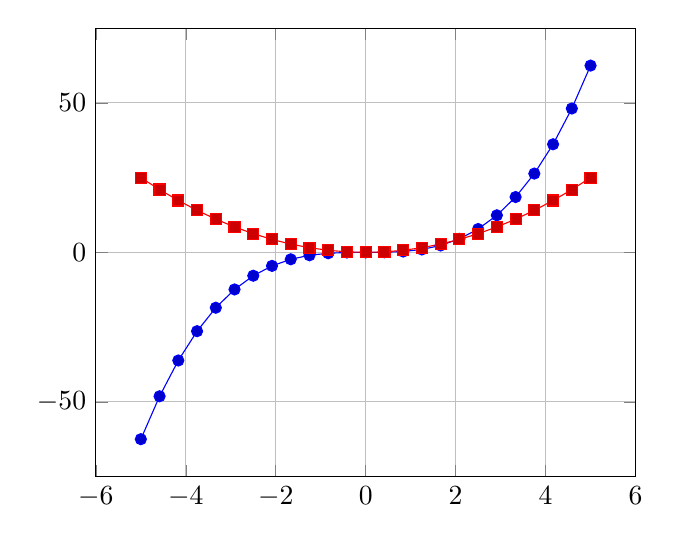
\begin{tikzpicture}
			\begin{axis}[grid=major, domain=-5:5]
				\addplot {(1/2)*x^3};
				\addplot {x^2};
			\end{axis}
		\end{tikzpicture}
		
		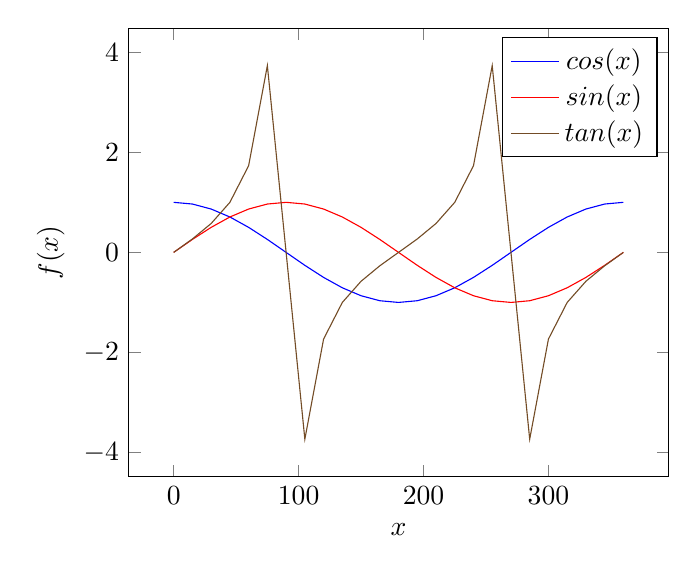
\begin{tikzpicture}
			\begin{axis}[domain=0:360, no markers, xlabel=$x$, ylabel=$f(x)$]
				\addplot {cos(x)};
				\addplot {sin(x)};
				\addplot {tan(x)};
				\legend{$cos(x)$, $sin(x)$,$tan(x)$}
			\end{axis}
		\end{tikzpicture}
	
	\section{Unités}
	
		La vitesse de la lumière est de \SI{3e8}{\m\per\second}.
		
		Nous sommes le jeudi 3 mai 2018 et la température est de \SI{13}{\celsius}.
		
	\section{Tableau de nombres}
	
		\begin{tabular}{|S|}
			\hline
			{Températures de la journée} \\
			\hline
			9.6 \\
			12 \\
			13.24 \\
			12.7835 \\
			\hline
		\end{tabular}

	

\end{document}
